\documentclass[tikz,border=3pt]{standalone}
\usepackage[utf8]{inputenc}
\usepackage[T1]{fontenc}
\usepackage{lmodern}
\renewcommand{\familydefault}{\sfdefault}
\usepackage{sansmath}\sansmath
\usepackage{chemfig}
\usepackage{pgfplots}\pgfplotsset{compat=1.18,/pgf/number format/use comma,/pgf/number format/1000 sep={.}}
\usetikzlibrary{arrows.meta,calc,positioning,decorations.pathmorphing,patterns}
% paleta del sitio
\definecolor{nar}{HTML}{E8680C}\definecolor{narc}{HTML}{FFB35C}\definecolor{hielo}{HTML}{FFF3E8}
\definecolor{tinta}{HTML}{1D1D1F}\definecolor{gris}{HTML}{6E6E73}\definecolor{lila}{HTML}{7C5CF0}
\definecolor{azul}{HTML}{2F6FD6}\definecolor{menta}{HTML}{17A673}\definecolor{coral}{HTML}{E8342A}
\tikzset{cel/.style={draw=gris,fill=hielo,line width=0.9pt},nuc/.style={draw=gris!70,line width=0.6pt},
fib/.style={gris!55,line width=0.35pt},eti/.style={font=\footnotesize,text=tinta,align=center},
num/.style={circle,draw=nar,fill=white,text=nar,font=\small\bfseries,inner sep=1.2pt,minimum size=13pt},
fl/.style={-{Stealth[length=2.6mm]},gris,line width=0.9pt}}
\begin{document}
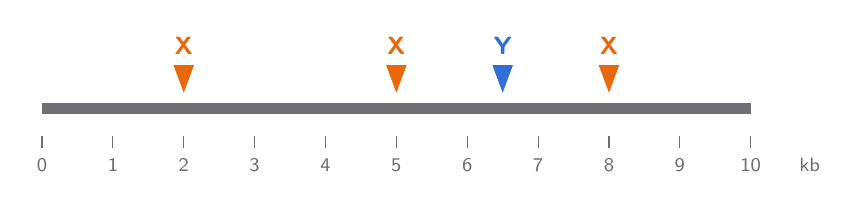
\begin{tikzpicture}[font=\small]
\draw[gris,line width=4pt] (0,0)--(9,0);
\draw[gris] (0,-0.35)--(0,-0.5);\node[font=\scriptsize,text=gris] at (0,-0.72) {0};
\draw[gris] (0.9,-0.35)--(0.9,-0.5);\node[font=\scriptsize,text=gris] at (0.9,-0.72) {1};
\draw[gris] (1.8,-0.35)--(1.8,-0.5);\node[font=\scriptsize,text=gris] at (1.8,-0.72) {2};
\draw[gris] (2.7,-0.35)--(2.7,-0.5);\node[font=\scriptsize,text=gris] at (2.7,-0.72) {3};
\draw[gris] (3.6,-0.35)--(3.6,-0.5);\node[font=\scriptsize,text=gris] at (3.6,-0.72) {4};
\draw[gris] (4.5,-0.35)--(4.5,-0.5);\node[font=\scriptsize,text=gris] at (4.5,-0.72) {5};
\draw[gris] (5.4,-0.35)--(5.4,-0.5);\node[font=\scriptsize,text=gris] at (5.4,-0.72) {6};
\draw[gris] (6.3,-0.35)--(6.3,-0.5);\node[font=\scriptsize,text=gris] at (6.3,-0.72) {7};
\draw[gris] (7.2,-0.35)--(7.2,-0.5);\node[font=\scriptsize,text=gris] at (7.2,-0.72) {8};
\draw[gris] (8.1,-0.35)--(8.1,-0.5);\node[font=\scriptsize,text=gris] at (8.1,-0.72) {9};
\draw[gris] (9,-0.35)--(9,-0.5);\node[font=\scriptsize,text=gris] at (9,-0.72) {10};
\node[font=\scriptsize,text=gris] at (9.75,-0.72) {kb};
\fill[nar] (1.67,0.55)--(1.93,0.55)--(1.8,0.2)--cycle;\node[font=\small\bfseries,text=nar] at (1.8,0.8) {X};
\fill[nar] (4.37,0.55)--(4.63,0.55)--(4.5,0.2)--cycle;\node[font=\small\bfseries,text=nar] at (4.5,0.8) {X};
\fill[nar] (7.07,0.55)--(7.33,0.55)--(7.2,0.2)--cycle;\node[font=\small\bfseries,text=nar] at (7.2,0.8) {X};
\fill[azul] (5.72,0.55)--(5.98,0.55)--(5.85,0.2)--cycle;\node[font=\small\bfseries,text=azul] at (5.85,0.8) {Y};
\end{tikzpicture}
\end{document}
